\documentclass[letter,11pt]{article}

\usepackage[spanish,es-nodecimaldot]{babel}
\usepackage[utf8]{inputenc}

\usepackage{lmodern}
\usepackage[T1]{fontenc}
\usepackage{textcomp}

\usepackage{framed}
\usepackage[svgnames]{xcolor}
\colorlet{shadecolor}{Gainsboro!50}

\usepackage[labelfont=bf]{caption}
\usepackage{graphicx}
\usepackage{pstricks}

\usepackage{anysize}
\marginsize{3cm}{2cm}{2cm}{3cm}

\usepackage{siunitx}
\usepackage{amsmath}
\usepackage{array}

\usepackage{fancyhdr}
\usepackage{lastpage}
\pagestyle{fancy}
\fancyhf{}
\fancyhead[LE,RO]{Laboratorio de Física Básica III}
\fancyfoot[CO,CE]{\thepage\ de \pageref{LastPage}}

\special{papersize=215.9mm,279.4mm}

\usepackage[
    pdfauthor={
        Bastos Lizondo Rosemary;
        Blanco Alconz John Brandon;
        Caballero Burgoa Carlos Eduardo;
        Villena Gutiérrez Ismael Cristian
    },%
    pdftitle={Laboratorio de Física Básica III},%
    pdfsubject={Carga y descarga de un capacitor},%
    colorlinks,%
    citecolor=black,%
    filecolor=black,%
    linkcolor=black,%
    urlcolor=black,
    breaklinks]{hyperref}
\usepackage{breakurl}

\newcommand{\blankpage}{
\newpage
\thispagestyle{empty}
\mbox{}
\newpage
}

\renewcommand{\arraystretch}{1.2}

\begin{document}

\begin{titlepage}
\begin{center}
{\Large UNIVERSIDAD MAYOR DE SAN SIMÓN}\\
\vspace*{0.15cm}
{\large FACULTAD DE CIENCIAS Y TECNOLOGÍA}\\
\vspace*{0.10cm}
DEPARTAMENTO DE FÍSICA\\
\vspace*{3.0cm}
{\Large \textbf{LABORATORIO DE FÍSICA BÁSICA III}}\\
\vspace*{0.3cm}
{\Large \textbf{INFORME No. 7}}\\
\vspace*{3.5cm}
{\Large \textbf{CARGA Y DESCARGA DE UN CAPACITOR}}\\
\end{center}

\vspace*{5.8cm}
\leftskip=7.95cm
\noindent
\textbf{Integrantes:}\\
Bastos Lizondo Rosemary.\\
Blanco Alconz John Brandon.\\
Caballero Burgoa Carlos Eduardo.\\
Villena Gutiérrez Ismael Cristian.\\
\newline
\textbf{Docente:}\\
Ing. Flores Flores, Freddy.\\
\newline
\textbf{Grupo:} G3.\\
\textbf{Fecha de entrega:} 20 de Mayo del 2021.\\

\end{titlepage}

\section{Evaluación previa}
\begin{enumerate}
\item \textbf{¿Qué es un capacitor (condensador) electrolítico?} \\
Un condensador electrolítico es un tipo de condensador que usa un líquido
iónico conductor como una de sus placas. Típicamente con más capacidad por
unidad de volumen que otros tipos de condensadores, son valiosos en circuitos
eléctricos con relativa alta corriente y baja frecuencia.

\item \textbf{¿Qué interpretación tiene la constante de tiempo en el circuito
RC?} \\
Cuando $t$ (valor del tiempo) es igual a la constante de tiempo $\tau$, el
exponente de $e$ se vuelve $- 1$, y el término exponencial es igual a $1/e$, o
aproximadamente $0.37$. La constante de tiempo determina qué tan rápido tiende a
cero la exponencial. Después de que una constante de tiempo ha pasado, el
voltaje ha disminuido hasta el $37\%$ de su valor inicial.

\item \textbf{¿Cómo se puede determinar experimentalmente la constante de tiempo
de un circuito RC?} \\
Para hallar la constante de tiempo se deben calcular los parámetros de la curva
tiempo vs. voltaje, en el proceso de carga o descarga de un condensador, y según
el caso usar la ecuación respectiva.

\item \textbf{¿Cómo se carga un capacitor?, escribir las ecuaciones.} \\
Al conectar un condensador en serie con una resistencia a una fuente de tensión
eléctrica (o comúnmente, fuente de alimentación), la corriente empieza a
circular por ambos. El condensador va acumulando carga entre sus placas. Cuando
el condensador se encuentra totalmente cargado, deja de circular corriente por
el circuito.

\begin{equation*}
    V(t) = V_o ( 1 - e^{-\frac{1}{RC}} )
\end{equation*}
\begin{equation*}
    I(t) = \frac{V_o}{R} e^{-\frac{1}{RC}}
\end{equation*}

\item \textbf{¿Cómo se descarga un capacitor?, escribir las ecuaciones.} \\
Si se quita la fuente y se coloca el condensador y la resistencia en paralelo,
las cargas empiezan a fluir de una de las placas del condensador a la otra a
través de la resistencia, hasta que la carga o energía almacenada en el
condensador es nula. En este caso, la corriente circulará en sentido contrario
al que circulaba mientras el condensador se estaba cargando.

\begin{equation*}
    V(t) = V_o e^{-\frac{1}{RC}}
\end{equation*}
\begin{equation*}
    I(t) = -\frac{V_o}{R} e^{-\frac{1}{RC}}
\end{equation*}
\end{enumerate}

\section{Objetivos}
\begin{itemize}
    \item Determinar la relación funcional entre el voltaje del capacitor y el
        tiempo para el proceso de carga del capacitor.
    \item Determinar la relación funcional entre el voltaje del capacitor y el
        tiempo para el proceso de descarga del capacitor.
    \item Determinar la constante de tiempo $\tau$ para el proceso de carga.
    \item Determinar la constante de tiempo $\tau$ para el proceso de descarga.
\end{itemize}

\section{Fundamento teórico}
Un capacitor es un dispositivo pasivo que tiene la función de almacenar energía
en forma de campo eléctrico.

\begin{figure}[!h]
\centering
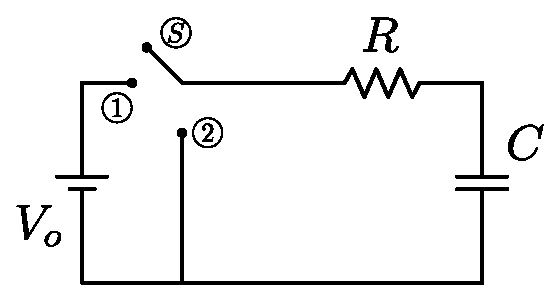
\includegraphics[scale=0.75]{resources/figura1.eps}
\caption{Circuito $RC$ para la carga y descarga del capacitor.}
\label{figura1}
\end{figure}

En la \textbf{Figura \ref{figura1}} se observa un circuito $RC$, donde el
capacitor y la resistencia están conectados en serie. Para que el capacitor
adquiera carga, el interruptor $S$ debe estar en la posición $1$, y para que el
capacitor se descargue, el interruptor $S$ debe estar en la posición $2$.

\subsection{Proceso de carga del capacitor}
Para el proceso de carga del capacitor, y con la segunda ley de
\emph{Kirchhoff}, se tiene:

\begin{equation}
    V_0 - V_R - V_C = 0
\label{carga1}
\end{equation}
\vspace{-0.1cm}

Donde $V_R = R\,I$, $V_C = Q/C$ y para la corriente $i = dQ/dt$, entonces la
\textbf{Ecuación \ref{carga1}} es:

\begin{equation}
    R \frac{dQ}{dt} + \frac{Q}{C} = V_0
\label{carga2}
\end{equation}
\vspace{-0.1cm}

Cuya solución es:

\begin{equation*}
    Q = C\,V_0 (1 - e^{-\frac{t}{RC}})
\end{equation*}
\vspace{-0.1cm}

Entonces, el voltaje en el capacitor es:

\begin{equation}
    V_c = \frac{Q}{C} = V_0 (1 - e^{-\frac{t}{RC}})
\label{carga3}
\end{equation}
\vspace{-0.1cm}

El producto $RC$ es una constante que tiene unidades de tiempo, y se conoce como
constante de tiempo $\tau$.

La corriente en el proceso de carga es:

\begin{equation}
    I = \frac{dQ}{dt} = \frac{V_0}{R}\,e^{-\frac{t}{RC}}
\label{carga4}
\end{equation}
\vspace{-0.1cm}

Con la ley de \emph{Ohm} y la \textbf{Ecuación \ref{carga4}}, se obtiene el
voltaje en la resistencia:

\begin{equation*}
    V_R = V_0\,e^{-\frac{t}{RC}}
\end{equation*}
\vspace{-0.1cm}

\subsection{Proceso de descarga del capacitor}
Para el proceso de descarga del capacitor, la fuente de tensión continua está
desconectada del circuito $RC$ (En la \textbf{Figura \ref{figura1}}, $s$ está en
la posición $2$). A partir de ello, la \textbf{Ecuación \ref{carga2}} es:

\begin{equation}
    R \frac{dQ}{dt} + \frac{Q}{C} = 0
\label{descarga1}
\end{equation}
\vspace{-0.1cm}

Cuya solución es:

\begin{equation*}
    Q = C\,V_0 e^{-\frac{t}{RC}}
\end{equation*}
\vspace{-0.1cm}

Entonces, el voltaje en el capacitor es:

\begin{equation}
    V_C = V_0\,e^{-\frac{t}{RC}}
\label{descarga2}
\end{equation}
\vspace{-0.1cm}

La corriente en el proceso de la descarga del capacitor es:

\begin{equation}
    I = -\frac{V_0}{R}\,e^{-\frac{t}{RC}}
\label{descarga3}
\end{equation}
\vspace{-0.1cm}

y con la \textbf{Ecuación \ref{descarga3}} el voltaje en la resistencia es:

\begin{equation*}
    V_R = -V_0\,e^{-\frac{t}{RC}}
\end{equation*}
\vspace{-0.1cm}

\section{Materiales}
\begin{itemize}
\item Simulador «PhET Interactive Simulations» Circuit Construction Kit: AC.
\end{itemize}

En el simulador se usarán los siguientes componentes:

\begin{itemize}
    \item Capacitor de $0.1 [F]$.
    \item Batería de $9.0 [V]$.
    \item Resistencia de $120 [\Omega]$.
    \item Voltímetro.
    \item Cronómetro.
    \item Cables de conexión.
\end{itemize}

\section{Procedimiento experimental}

\subsection{Carga del capacitor}
A continuación se describe el procedimiento experimental que se llevará a cabo.

\begin{figure}[!h]
\centering
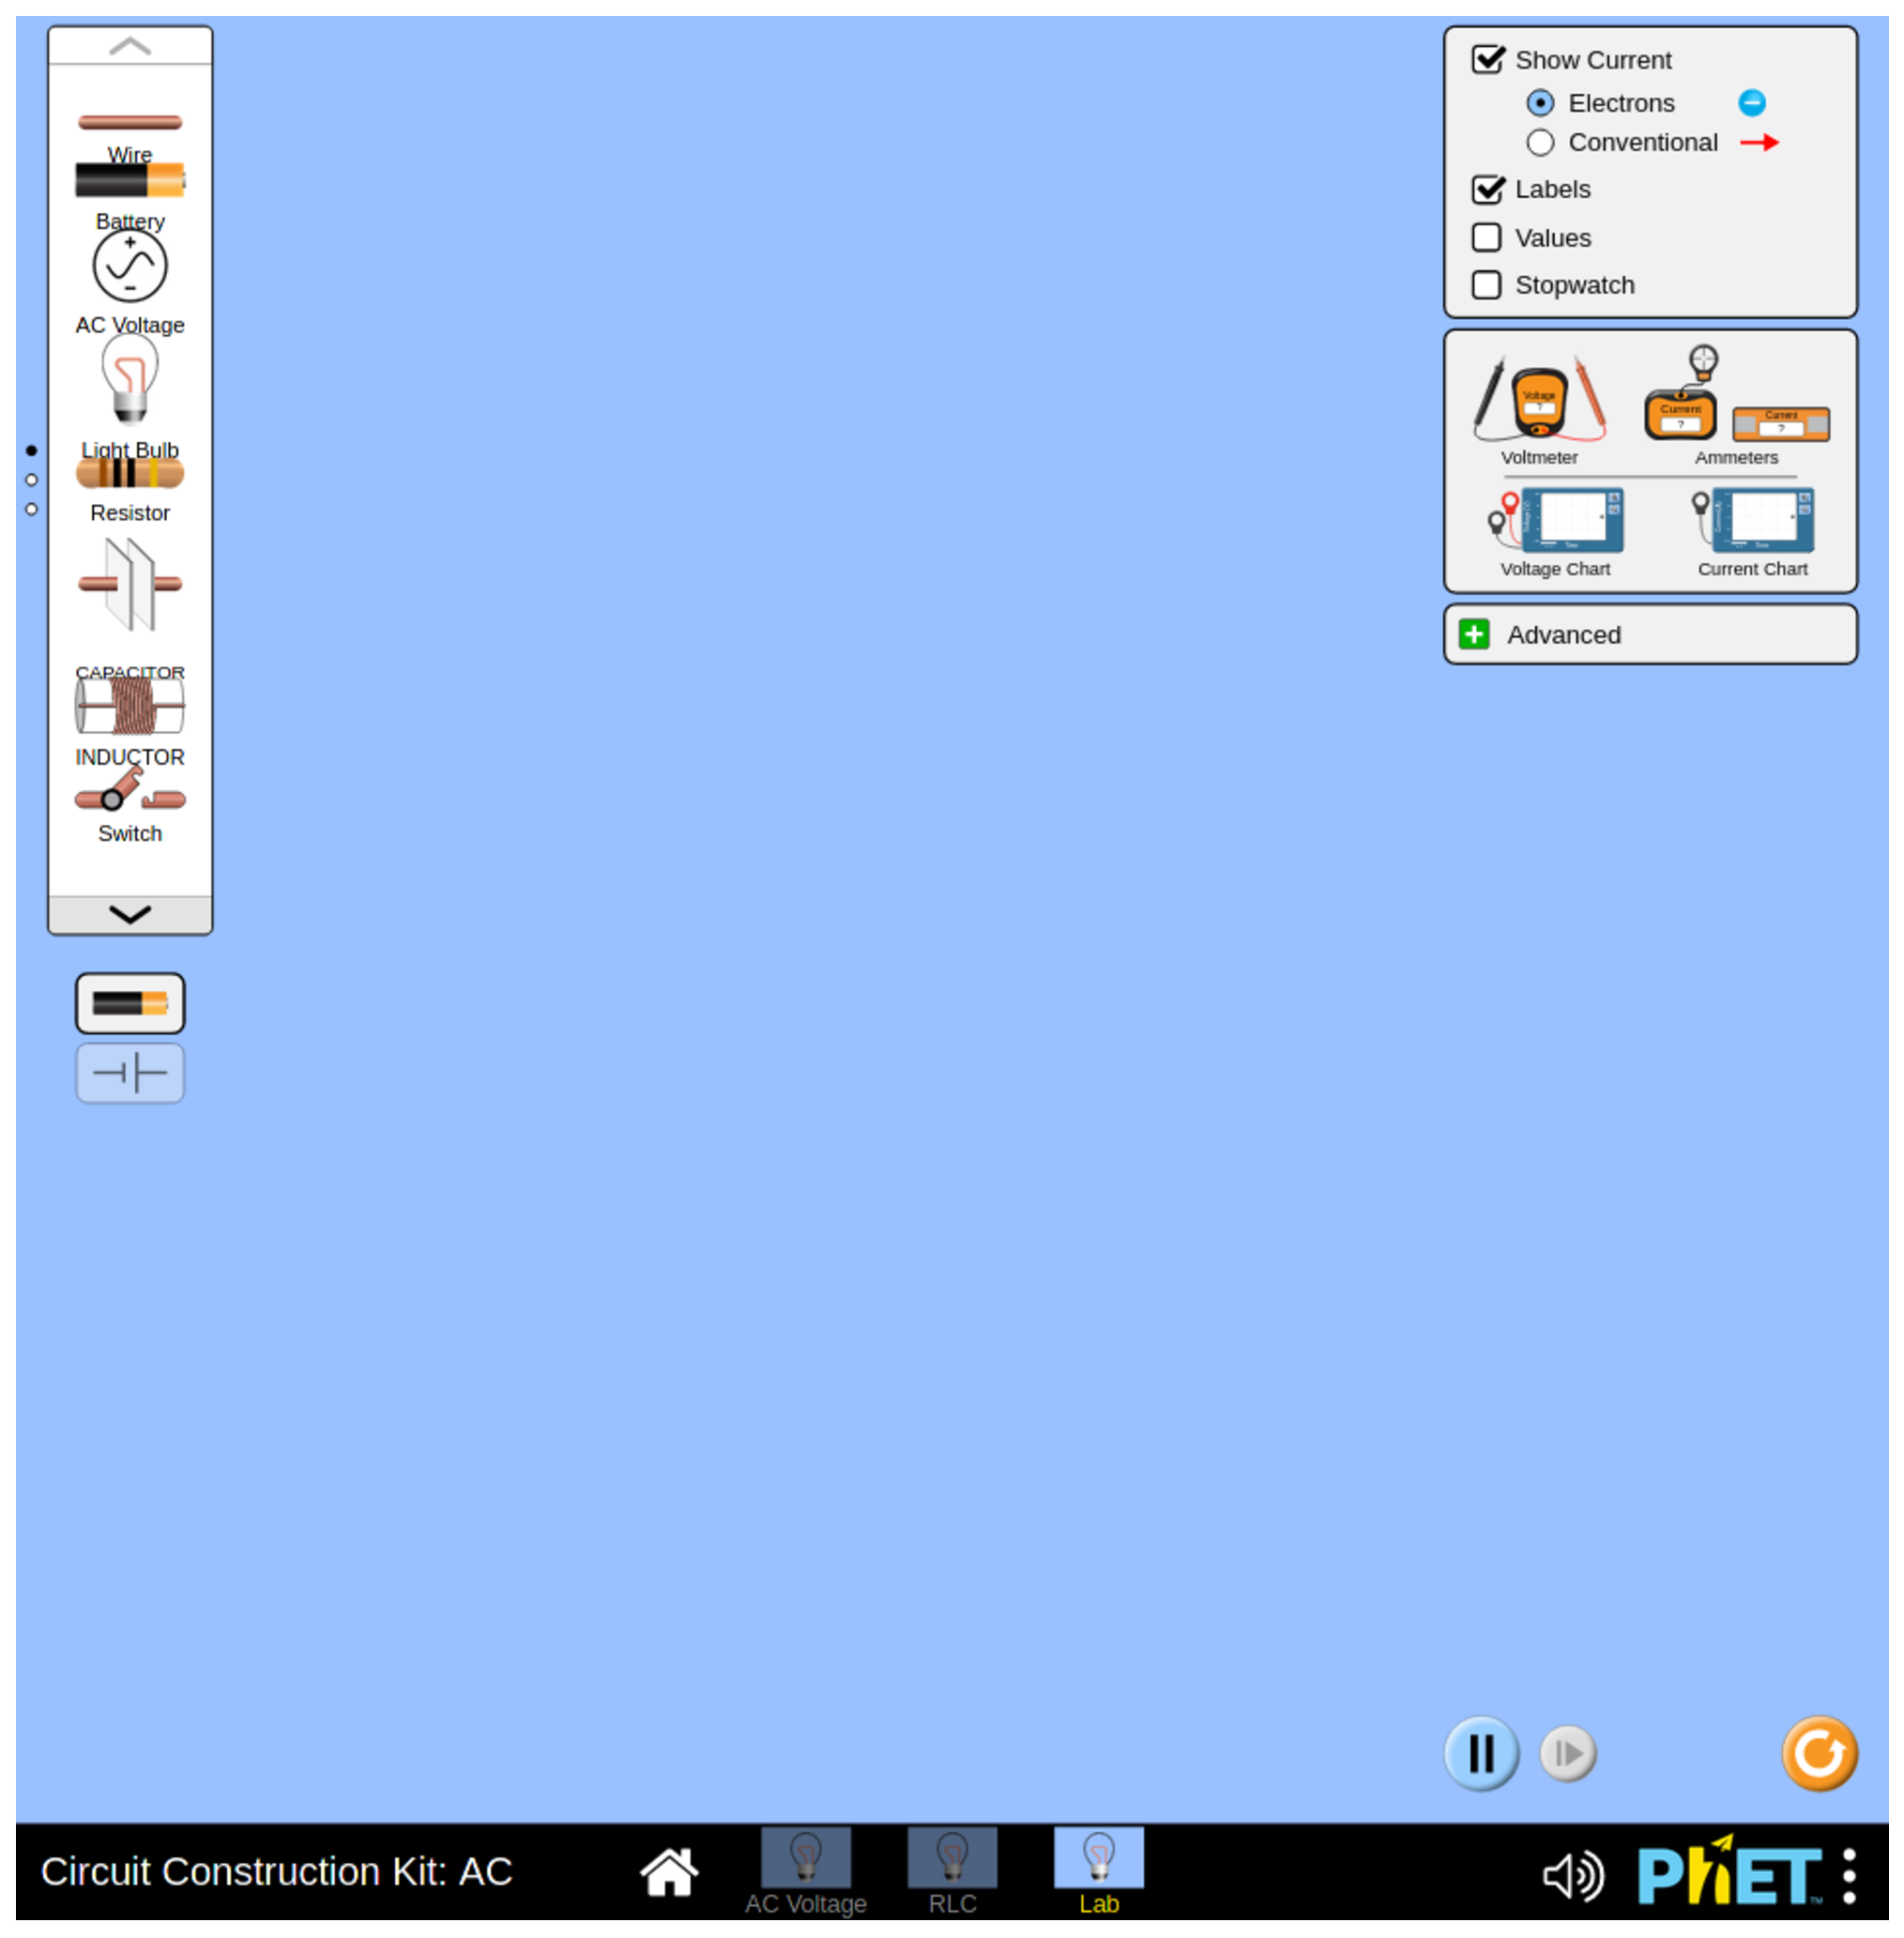
\includegraphics[scale=0.40]{resources/figura2.eps}
\caption{Simulador para el montaje de circuitos.}
\label{figura2}
\end{figure}

\begin{enumerate}
\item Ir al simulador ubicado en la dirección web:
(https://phet.colorado.edu/sims/html/circuit-construction-kit-ac/latest/circuit-construction-kit-ac\_en.html),
tal como se muestra en la \textbf{Figura \ref{figura2}}.
\item Armar el circuito tal como se muestra en la \textbf{Figura \ref{figura1}}.
\item Conectar el voltímetro para la medición del voltaje en el capacitor.
\item Conectar el interruptor $S$ en la posición $1$.
\item Paralelamente al paso anterior, cronometrar los tiempos transcurridos para
    diferentes valores del voltaje marcado por el voltímetro.
\item Registrar las mediciones tomadas, elaborar las gráficas e interpretar los
    resultados.
\end{enumerate}

\subsection{Descarga del capacitor}
A continuación se describe el procedimiento experimental que se llevará a cabo.

\begin{enumerate}
\item Ir al simulador ubicado en la dirección web:
(https://phet.colorado.edu/sims/html/circuit-construction-kit-ac/latest/circuit-construction-kit-ac\_en.html),
tal como se muestra en la \textbf{Figura \ref{figura2}}.
\item Armar el circuito tal como se muestra en la \textbf{Figura \ref{figura1}}.
\item Conectar el voltímetro para la medición del voltaje en el capacitor.
\item Cargar el capacitor hasta su máxima capacidad.
\item Conectar el interruptor $S$ en la posición $2$.
\item Paralelamente al paso anterior, cronometrar los tiempos transcurridos para
    diferentes valores del voltaje marcado por el voltímetro.
\item Registrar las mediciones tomadas, elaborar las gráficas e interpretar los
    resultados.
\end{enumerate}

\section{Resultados}

\begin{figure}[!h]
\centering
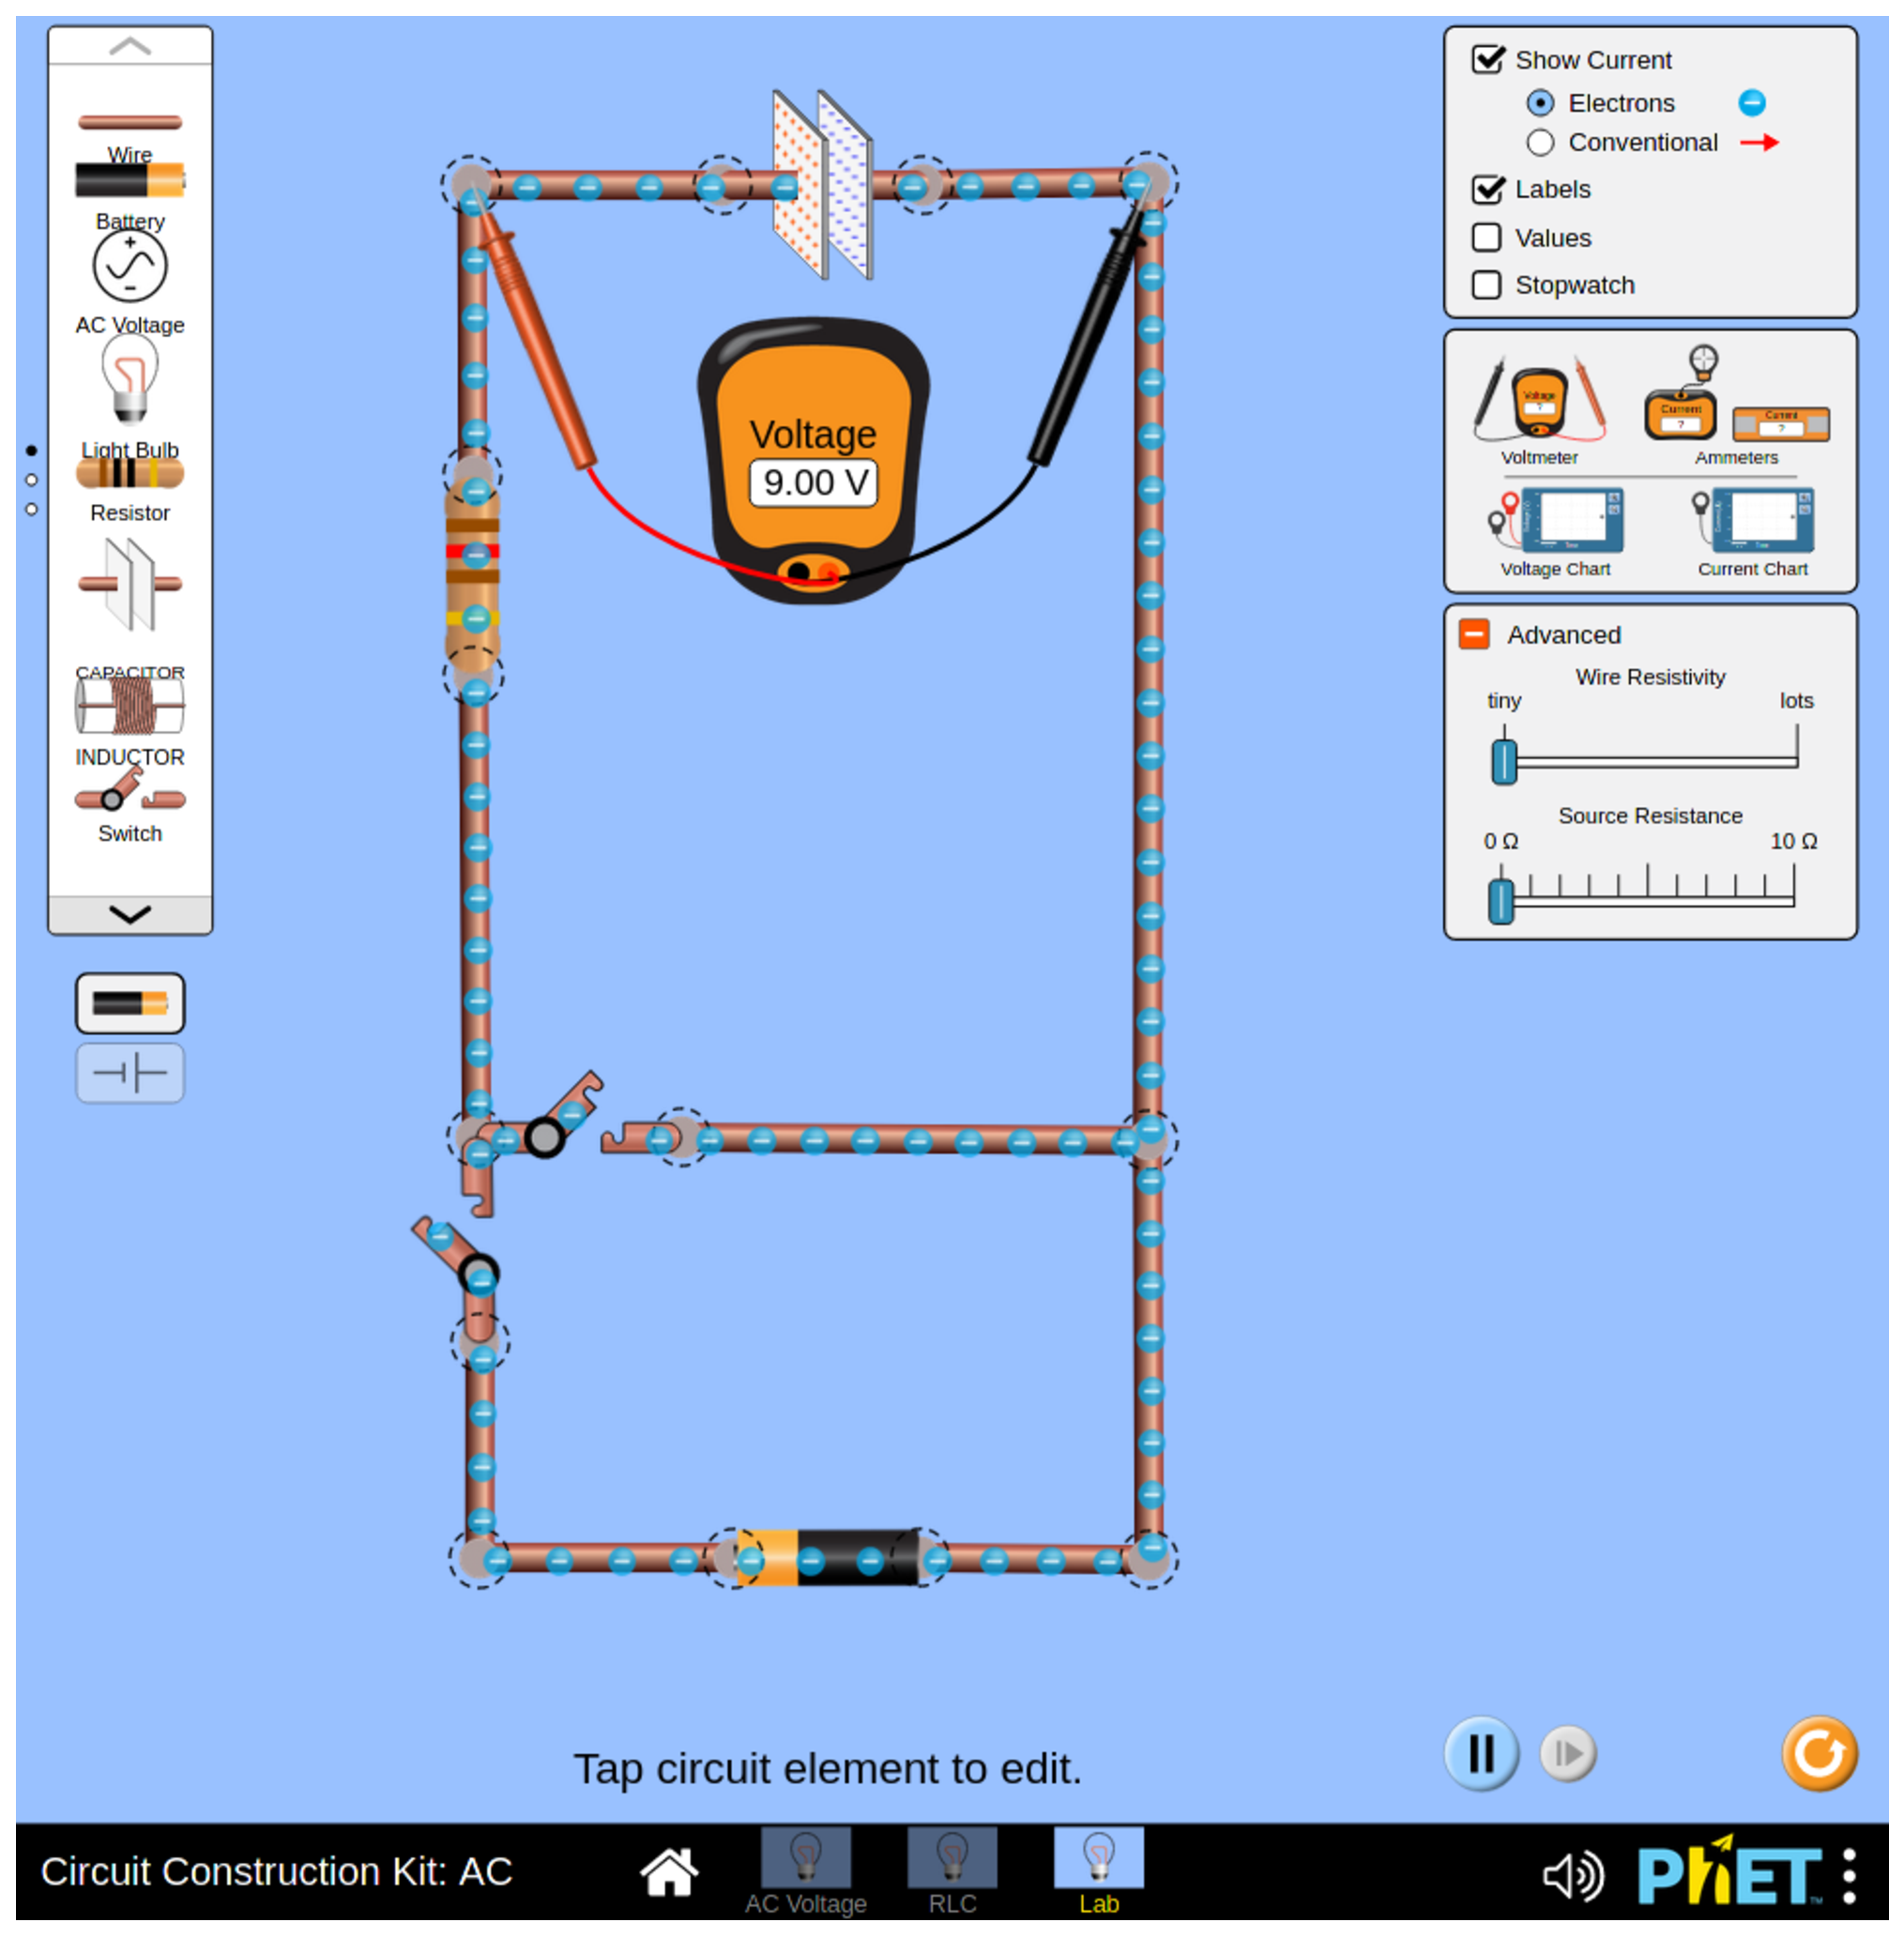
\includegraphics[scale=0.40]{resources/figura3.eps}
\caption{Circuito usado para el experimento.}
\label{figura3}
\end{figure}

En la \textbf{Figura \ref{figura3}} se presenta el armado del circuito realizado
en el simulador.

Voltaje de la batería:

\begin{equation*}
    V = 9.0 [V]
\end{equation*}

Resistencia del circuito:

\begin{equation*}
    R = 120.0 [\Omega]
\end{equation*}

Capacitancia del condensador:

\begin{equation*}
    C = 0.1 [F]
\end{equation*}

\subsection{Carga del capacitor}
En el \textbf{Cuadro \ref{cuadro1}} se presentan los valores del tiempo
cronometrado, y el tiempo absoluto para determinados valores de voltaje.

\begin{table}[!h]
\begin{center}
\begin{tabular}{|c||>{\centering}m{3.0cm}<{\centering}|
                  |>{\centering}m{1.2cm}<{\centering}
                  |>{\centering}m{1.2cm}<{\centering}|}
\hline
$i$ & Cronometrado & $t_i [s]$ & $V_i [V]$ \tabularnewline \hline \hline
 1 & 00:04.37 &  0    & 0.05 \tabularnewline \hline
 2 & 00:05.72 &  1.35 & 1.00 \tabularnewline \hline
 3 & 00:07.33 &  2.96 & 2.01 \tabularnewline \hline
 4 & 00:09.16 &  4.79 & 3.00 \tabularnewline \hline
 5 & 00:11.38 &  7.01 & 4.01 \tabularnewline \hline
 6 & 00:14.03 &  9.66 & 5.00 \tabularnewline \hline
 7 & 00:17.53 & 13.16 & 6.01 \tabularnewline \hline
 8 & 00:22.33 & 17.96 & 7.00 \tabularnewline \hline
 9 & 00:30.63 & 26.26 & 8.00 \tabularnewline \hline
10 & 01:34.26 & 89.89 & 9.00 \tabularnewline \hline
\end{tabular}
\caption{Mediciones del voltaje y tiempo de carga del capacitor.}
\label{cuadro1}
\end{center}
\end{table}

\begin{figure}[!h]
\centering
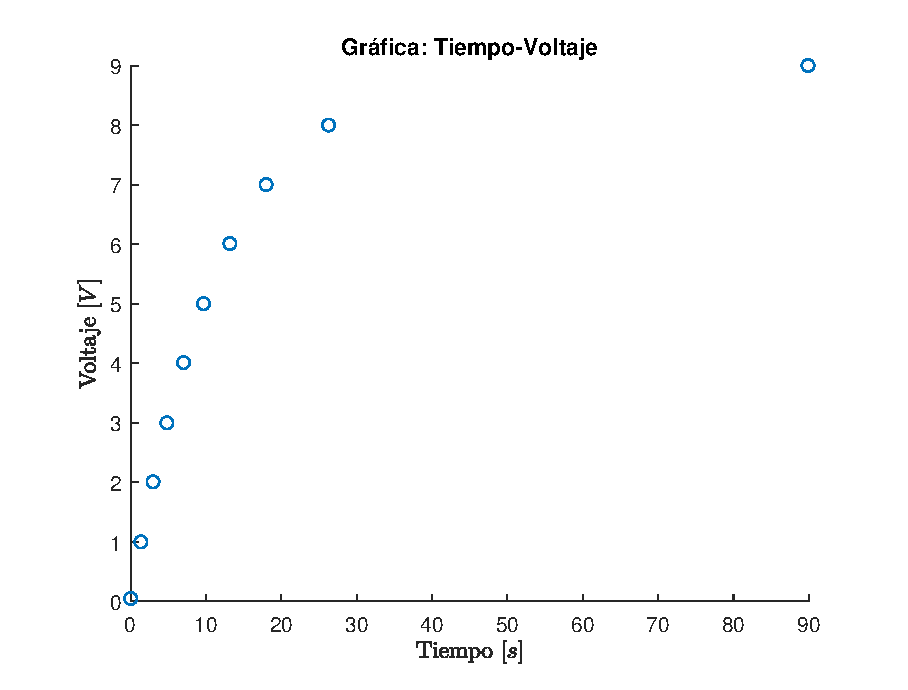
\includegraphics[scale=1.00]{resources/m1.1.eps}
\caption{Voltaje del capacitor en función del tiempo (Carga).}
\label{figura4}
\end{figure}

A partir de los datos del \textbf{Cuadro \ref{cuadro1}}, se obtiene la gráfica
presentada en la \textbf{Figura \ref{figura4}}.

Por la forma de la \textbf{Figura \ref{figura4}} y considerando la
\textbf{Ecuación \ref{carga3}}:

\begin{equation*}
    V = V_0 ( 1 - e^{-\frac{t}{\tau}} )
\end{equation*}

Despejando $t$ obtenemos:

\begin{equation*}
    V = V_0 - V_0\,e^{-\frac{t}{\tau}}
\end{equation*}
\begin{equation*}
    V - V_0 = -V_0\,e^{-\frac{t}{\tau}}
\end{equation*}
\begin{equation*}
    -\frac{V - V_0}{V_0} = e^{-\frac{t}{\tau}}
\end{equation*}

Aplicando logaritmos naturales a ambos lados de la ecuación:

\begin{equation*}
    ln \left(1 - \frac{V}{V_0}\right) = - \frac{1}{\tau} t
\end{equation*}

Haciendo los siguientes cambios de variables:

\begin{equation*}
    V' = ln \left(1 - \frac{V}{V_0}\right)
\end{equation*}
\begin{equation}
    B = -\frac{1}{\tau}
\label{tiempo1}
\end{equation}
\begin{equation*}
    t' = t
\end{equation*}

Se obtiene:

\begin{equation*}
    V' = A + B t'
\end{equation*}

En el \textbf{Cuadro \ref{cuadro2}} pueden apreciarse los valores de la función
aplicando los cambios de variable respectivos, tales datos generan la gráfica
presentada en la \textbf{Figura \ref{figura5}}.

\begin{table}[!h]
\begin{center}
\begin{tabular}{|c||>{\centering}m{2.0cm}<{\centering}
                  |>{\centering}m{2.0cm}<{\centering}|}
\hline
$i$ & $t'_i$ & $V'_i$ \tabularnewline \hline \hline
1 &  0    & -0.0056 \tabularnewline \hline
2 &  1.35 & -0.1178 \tabularnewline \hline
3 &  2.96 & -0.2527 \tabularnewline \hline
4 &  4.79 & -0.4055 \tabularnewline \hline
5 &  7.01 & -0.5898 \tabularnewline \hline
6 &  9.66 & -0.8109 \tabularnewline \hline
7 & 13.16 & -1.1020 \tabularnewline \hline
8 & 17.96 & -1.5041 \tabularnewline \hline
9 & 26.26 & -2.1972 \tabularnewline \hline
\end{tabular}
\caption{Valores después del cambio de variable.}
\label{cuadro2}
\end{center}
\end{table}

\begin{figure}[!h]
\centering
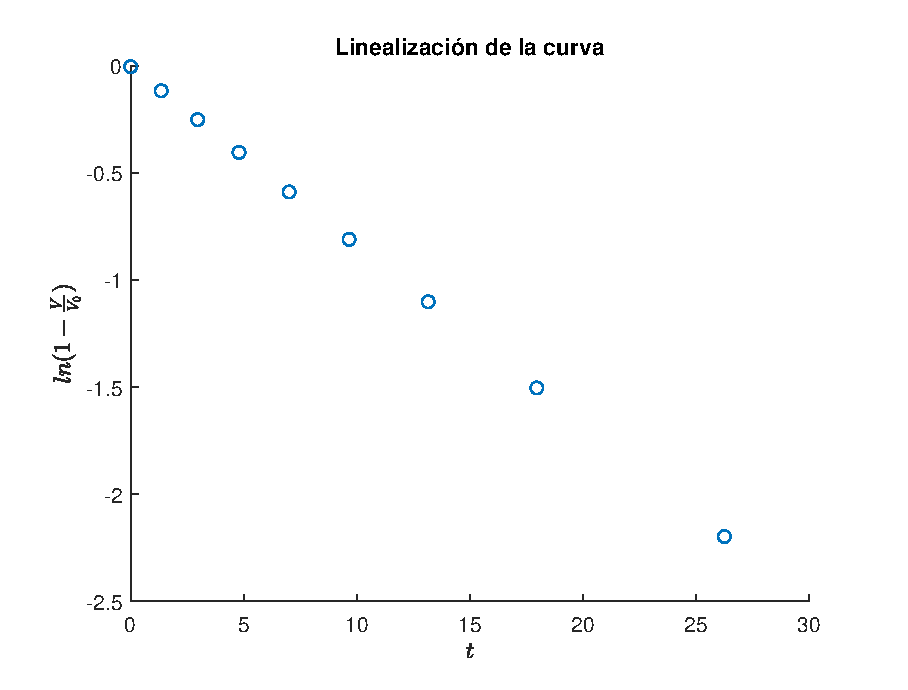
\includegraphics[scale=1.00]{resources/m1.2.eps}
\caption{Gráfica de la función linealizada.}
\label{figura5}
\end{figure}

Se calcularon los parámetros de la recta por el método de los mínimos cuadrados,
con la ayuda de los datos presentados en el \textbf{Cuadro \ref{cuadro3}}.

\begin{table}[!h]
\begin{center}
\begin{tabular}{|c||>{\centering}m{1.6cm}<{\centering}
                   |>{\centering}m{1.6cm}<{\centering}
                   |>{\centering}m{1.6cm}<{\centering}|
                   |>{\centering}m{1.8cm}<{\centering}
                   |>{\centering}m{1.8cm}<{\centering}
                   |>{\centering}m{1.8cm}<{\centering}|}
\hline
$i$ & $t'_i V'_i$ & $t'^2_i$ & $V'^2_i$ & $Y$ & $d_i$ & $d^2_i (\num{e-5})$
    \tabularnewline \hline \hline
1 &        0 &        0 & 0.0000 & -0.0052 & -0.0004 & 0.0127 \tabularnewline \hline
2 &  -0.1590 &   1.8225 & 0.0139 & -0.1179 &  0.0001 & 0.0007 \tabularnewline \hline
3 &  -0.7481 &   8.7616 & 0.0639 & -0.2522 & -0.0005 & 0.0278 \tabularnewline \hline
4 &  -1.9422 &  22.9441 & 0.1644 & -0.4049 & -0.0005 & 0.0292 \tabularnewline \hline
5 &  -4.1344 &  49.1401 & 0.3479 & -0.5902 &  0.0004 & 0.0151 \tabularnewline \hline
6 &  -7.8336 &  93.3156 & 0.6576 & -0.8113 &  0.0004 & 0.0145 \tabularnewline \hline
7 & -14.5017 & 173.1856 & 1.2143 & -1.1034 &  0.0014 & 0.2027 \tabularnewline \hline
8 & -27.0132 & 322.5616 & 2.2622 & -1.5039 & -0.0002 & 0.0025 \tabularnewline \hline
9 & -57.6991 & 689.5876 & 4.8278 & -2.1965 & -0.0007 & 0.0484 \tabularnewline \hline
\end{tabular}
\caption{Valores para el método de mínimos cuadrados.}
\label{cuadro3}
\end{center}
\end{table}

\begin{equation*}
    n = 9
\end{equation*}
\begin{equation*}
    \sum t'_i = 83.1500
\end{equation*}
\begin{equation*}
    \sum V'_i = -6.9855
\end{equation*}
\begin{equation*}
    \sum t'^2_i = \num{1.3613e3}
\end{equation*}
\begin{equation*}
    \sum V'^2_i = 9.5520
\end{equation*}
\begin{equation*}
    \sum t'_i V'_i = -114.0313
\end{equation*}
\begin{equation*}
    \Delta_1 = n \sum I^2_i - \left( \sum I_i \right)^2 = \num{5.3379e3}
\end{equation*}
\begin{equation*}
    \Delta_2 = n \sum V^2_i - \left( \sum V_i \right)^2 = 37.1702
\end{equation*}
\begin{equation*}
    A = \frac{\sum V_i \sum I^2_i - \sum I_i V_i \sum I_i}{\Delta_1} = -0.0052
\end{equation*}
\begin{equation*}
    B = \frac{n \sum I_i V_i - \sum I_i \sum V_i}{\Delta_1} = -0.0834
\end{equation*}
\begin{equation*}
    \sum d^2 = \num{3.5358e-6}
\end{equation*}
\begin{equation*}
    \sigma^2 = \frac{\sum d^2_i}{n-2} = \num{5.0511e-7}
\end{equation*}
\begin{equation*}
    \sigma_A = \sqrt{\frac{\sigma^2 \sum d^2_i}{\Delta_1}} = \num{3.5891e-4}
\end{equation*}
\begin{equation*}
    \sigma_B = \sqrt{\frac{\sigma^2 n}{\Delta_1}} = \num{2.9183e-5}
\end{equation*}

\begin{equation*}
    A = (-0.0052 \pm 0.0004)[u]; 6.88 \%
\end{equation*}
\begin{equation*}
    B = (-0.0834 \pm 0.00003)[s^{-1}]; 0.03 \%
\end{equation*}

Siendo el coeficiente de correlación:

\begin{equation*}
    r = \frac{n \sum I_i V_i - (\sum I_i)(\sum V_i)}{\sqrt{\Delta_1 \Delta_2}} = -1.0000
\end{equation*}

La ecuación de la recta resultante es:

\begin{equation*}
    V' = -0.0052 - 0.0834 \cdot t'
\end{equation*}

Por tanto, se comprueba la relación entre el voltaje y el tiempo para el proceso
de carga del capacitor descrito por la \textbf{Ecuación \ref{carga3}}.

\begin{center}
\begin{tabular}{|>{\centering}m{9.2cm}<{\centering}|}
\hline
\textbf{Resultado} 
\tabularnewline \hline
\\
\Large{$V(t) = 9 \left( 1 - e^{-\frac{1}{RC}\,t} \right) $} \tabularnewline
\\
\hline
\end{tabular}
\end{center}

Se determinará la constante de tiempo $\tau$, a partir de la
\textbf{Ecuación \ref{tiempo1}}:

\begin{equation*}
    \tau = - \frac{1}{B} = 11.9837 [s]
\end{equation*}

La derivada parcial es:

\begin{equation*}
    \frac{\partial \tau}{\partial B} = \frac{1}{B^2}
\end{equation*}

Siendo el error de la medición:

\begin{equation*}
    e_{\tau} = \Biggr| \frac{1}{B^2}\,e_B \Biggr| = 0.0042
\end{equation*}

Por tanto la constante de tiempo es:

\begin{center}
\begin{tabular}{|>{\centering}m{12.0cm}<{\centering}|}
\hline
\textbf{Resultado}
\tabularnewline \hline
\\
    $\tau = (11.984 \pm 0.004)[s]; 0.03\%$ \tabularnewline
\\
\hline
\end{tabular}
\end{center}

\subsection{Descarga del capacitor}
En el \textbf{Cuadro \ref{cuadro4}} se presentan los valores del tiempo
cronometrado, y el tiempo absoluto para determinados valores de voltaje.

\begin{table}[!h]
\begin{center}
\begin{tabular}{|c||>{\centering}m{3.0cm}<{\centering}|
                  |>{\centering}m{1.2cm}<{\centering}
                  |>{\centering}m{1.2cm}<{\centering}|}
\hline
$i$ & Cronometrado & $t_i [s]$ & $V_i [V]$ \tabularnewline \hline \hline
 1 & 00:05.08 &   0    & 8.98 \tabularnewline \hline
 2 & 00:06.47 &   1.39 & 7.99 \tabularnewline \hline
 3 & 00:08.08 &   3.00 & 6.99 \tabularnewline \hline
 4 & 00:09.94 &   4.86 & 5.99 \tabularnewline \hline
 5 & 00:12.12 &   7.04 & 5.00 \tabularnewline \hline
 6 & 00:14.78 &   9.70 & 4.00 \tabularnewline \hline
 7 & 00:18.22 &  13.14 & 3.00 \tabularnewline \hline
 8 & 00:23.10 &  18.02 & 2.00 \tabularnewline \hline
 9 & 00:31.37 &  26.29 & 1.00 \tabularnewline \hline
10 & 02:02.65 & 117.57 & 0    \tabularnewline \hline
\end{tabular}
\caption{Mediciones del voltaje y tiempo de descarga del capacitor.}
\label{cuadro4}
\end{center}
\end{table}

\begin{figure}[!h]
\centering
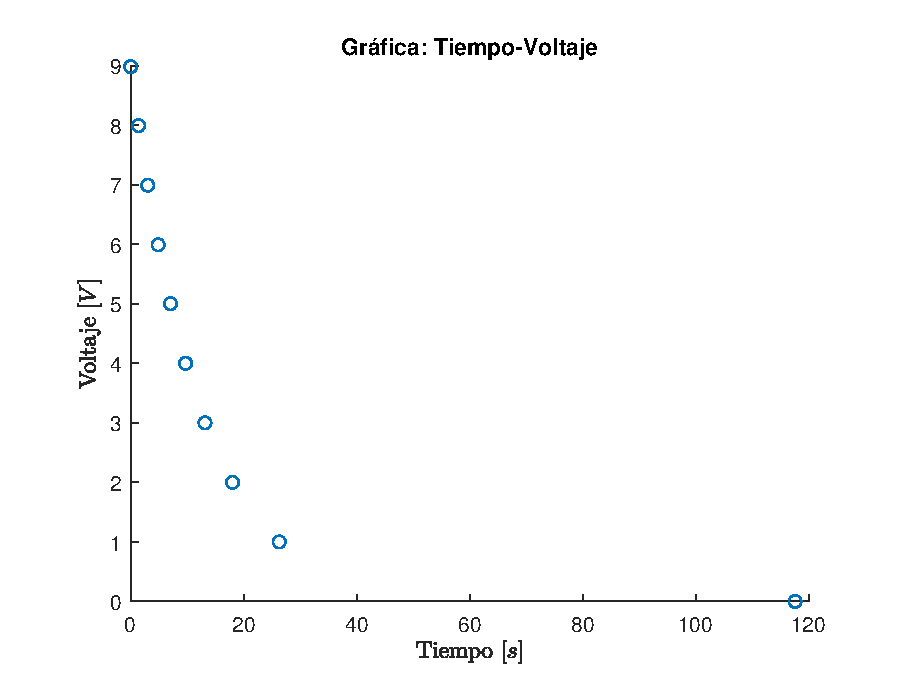
\includegraphics[scale=1.00]{resources/m2.1.eps}
\caption{Voltaje del capacitor en función del tiempo (Descarga).}
\label{figura6}
\end{figure}

A partir de los datos del \textbf{Cuadro \ref{cuadro4}}, se obtiene la gráfica
presentada en la \textbf{Figura \ref{figura6}}.

Por la forma de la \textbf{Figura \ref{figura6}} y considerando la
\textbf{Ecuación \ref{descarga2}}:

\begin{equation*}
    V = V_0\,e^{-\frac{t}{\tau}}
\end{equation*}

Aplicando logaritmos naturales a ambos lados de la ecuación:

\begin{equation*}
    ln\,V = ln\,V_0 - \frac{1}{\tau}\,t
\end{equation*}

Haciendo los siguientes cambios de variables:

\begin{equation*}
    V' = ln\,V
\end{equation*}
\begin{equation*}
    A = ln\,V_0
\end{equation*}
\begin{equation}
    B = -\frac{1}{\tau}
\label{tiempo2}
\end{equation}
\begin{equation*}
    t' = t
\end{equation*}

Se obtiene:

\begin{equation*}
    V' = A + B t'
\end{equation*}

En el \textbf{Cuadro \ref{cuadro5}} pueden apreciarse los valores de la función
aplicando los cambios de variable respectivos, tales datos generan la gráfica
presentada en la \textbf{Figura \ref{figura7}}.

\begin{table}[!h]
\begin{center}
\begin{tabular}{|c||>{\centering}m{2.0cm}<{\centering}
                  |>{\centering}m{2.0cm}<{\centering}|}
\hline
$i$ & $t'_i$ & $V'_i$ \tabularnewline \hline \hline
1 &  0    & 2.1950 \tabularnewline \hline
2 &  1.39 & 2.0782 \tabularnewline \hline
3 &  3.00 & 1.9445 \tabularnewline \hline
4 &  4.86 & 1.7901 \tabularnewline \hline
5 &  7.04 & 1.6094 \tabularnewline \hline
6 &  9.70 & 1.3863 \tabularnewline \hline
7 & 13.14 & 1.0986 \tabularnewline \hline
8 & 18.02 & 0.6931 \tabularnewline \hline
9 & 26.29 &      0 \tabularnewline \hline
\end{tabular}
\caption{Valores después del cambio de variable.}
\label{cuadro5}
\end{center}
\end{table}

\begin{figure}[!h]
\centering
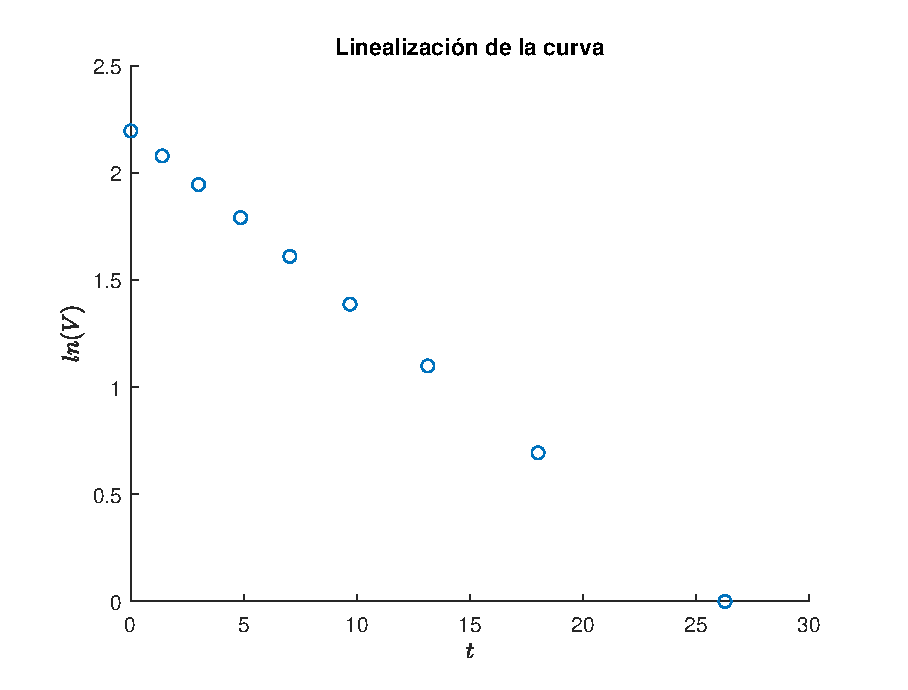
\includegraphics[scale=1.00]{resources/m2.2.eps}
\caption{Gráfica de la función linealizada.}
\label{figura7}
\end{figure}

Se calcularon los parámetros de la recta por el método de los mínimos cuadrados,
con la ayuda de los datos presentados en el \textbf{Cuadro \ref{cuadro6}}.

\begin{table}[!h]
\begin{center}
\begin{tabular}{|c||>{\centering}m{1.6cm}<{\centering}
                   |>{\centering}m{1.6cm}<{\centering}
                   |>{\centering}m{1.6cm}<{\centering}|
                   |>{\centering}m{1.8cm}<{\centering}
                   |>{\centering}m{1.8cm}<{\centering}
                   |>{\centering}m{1.8cm}<{\centering}|}
\hline
$i$ & $t'_i V'_i$ & $t'^2_i$ & $V'^2_i$ & $Y$ & $d_i$ & $d^2_i (\num{e-5})$
    \tabularnewline \hline \hline
1 &       0 &        0 & 4.8180 & 2.1954 & -0.0004 & 0.0146 \tabularnewline \hline
2 &  2.8887 &   1.9321 & 4.3189 & 2.0794 & -0.0012 & 0.1424 \tabularnewline \hline
3 &  5.8334 &   9.0000 & 3.7810 & 1.9450 & -0.0005 & 0.0299 \tabularnewline \hline
4 &  8.6998 &  23.6196 & 3.2044 & 1.7898 &  0.0003 & 0.0080 \tabularnewline \hline
5 & 11.3304 &  49.5616 & 2.5903 & 1.6079 &  0.0016 & 0.2414 \tabularnewline \hline
6 & 13.4471 &  94.0900 & 1.9218 & 1.3859 &  0.0004 & 0.0153 \tabularnewline \hline
7 & 14.4358 & 172.6596 & 1.2069 & 1.0988 & -0.0002 & 0.0048 \tabularnewline \hline
8 & 12.4905 & 324.7204 & 0.4805 & 0.6916 &  0.0016 & 0.2429 \tabularnewline \hline
9 &       0 & 691.1641 &      0 & 0.0014 & -0.0014 & 0.2091 \tabularnewline \hline
\end{tabular}
\caption{Valores para el método de mínimos cuadrados.}
\label{cuadro6}
\end{center}
\end{table}

\begin{equation*}
    n = 9
\end{equation*}
\begin{equation*}
    \sum t'_i = 83.4400
\end{equation*}
\begin{equation*}
    \sum V'_i = 12.7953
\end{equation*}
\begin{equation*}
    \sum t'^2_i = \num{1.3667e3}
\end{equation*}
\begin{equation*}
    \sum V'^2_i = 22.3218
\end{equation*}
\begin{equation*}
    \sum t'_i V'_i = 69.1257
\end{equation*}
\begin{equation*}
    \Delta_1 = n \sum I^2_i - \left( \sum I_i \right)^2 = \num{5.3385e3}
\end{equation*}
\begin{equation*}
    \Delta_2 = n \sum V^2_i - \left( \sum V_i \right)^2 = 37.1780
\end{equation*}
\begin{equation*}
    A = \frac{\sum V_i \sum I^2_i - \sum I_i V_i \sum I_i}{\Delta_1} = 2.1954
\end{equation*}
\begin{equation*}
    B = \frac{n \sum I_i V_i - \sum I_i \sum V_i}{\Delta_1} = -0.0835
\end{equation*}
\begin{equation*}
    \sum d^2 = \num{9.0844e-6}
\end{equation*}
\begin{equation*}
    \sigma^2 = \frac{\sum d^2_i}{n-2} = \num{1.2978e-6}
\end{equation*}
\begin{equation*}
    \sigma_A = \sqrt{\frac{\sigma^2 \sum d^2_i}{\Delta_1}} = \num{5.7641e-4}
\end{equation*}
\begin{equation*}
    \sigma_B = \sqrt{\frac{\sigma^2 n}{\Delta_1}} = \num{4.6775e-5}
\end{equation*}

\begin{equation*}
    A = (2.1954 \pm 0.0006)[u]; 0.03 \%
\end{equation*}
\begin{equation*}
    B = (-0.0835 \pm 0.00005)[s^{-1}]; 0.06 \%
\end{equation*}

Siendo el coeficiente de correlación:

\begin{equation*}
    r = \frac{n \sum I_i V_i - (\sum I_i)(\sum V_i)}{\sqrt{\Delta_1 \Delta_2}} = -1.0000
\end{equation*}

La ecuación de la recta resultante es:

\begin{equation*}
    V' = 2.1954 - 0.0835 \cdot t'
\end{equation*}

Por tanto, se comprueba la relación entre el voltaje y el tiempo para el proceso
de descarga del capacitor descrito por la \textbf{Ecuación \ref{descarga2}}.

\begin{center}
\begin{tabular}{|>{\centering}m{9.2cm}<{\centering}|}
\hline
\textbf{Resultado} 
\tabularnewline \hline
\\
\Large{$V(t) = 9\,e^{-\frac{1}{RC}\,t}$} \tabularnewline
\\
\hline
\end{tabular}
\end{center}

Se determinará la constante de tiempo $\tau$, a partir de la
\textbf{Ecuación \ref{tiempo2}}:

\begin{equation*}
    \tau = - \frac{1}{B} = 11.9830 [s]
\end{equation*}

La derivada parcial es:

\begin{equation*}
    \frac{\partial \tau}{\partial B} = \frac{1}{B^2}
\end{equation*}

Siendo el error de la medición:

\begin{equation*}
    e_{\tau} = \Biggr| \frac{1}{B^2}\,e_B \Biggr| = 0.0067
\end{equation*}

Por tanto la constante de tiempo es:

\begin{center}
\begin{tabular}{|>{\centering}m{12.0cm}<{\centering}|}
\hline
\textbf{Resultado}
\tabularnewline \hline
\\
    $\tau = (11.983 \pm 0.007)[s]; 0.05\%$ \tabularnewline
\\
\hline
\end{tabular}
\end{center}

\section{Cuestionario}
\begin{enumerate}
\item \textbf{Demostrar que la constante de tiempo $RC$, tiene unidades de
tiempo.} \\
Analizando sus unidades:

\begin{equation*}
    RC = [\Omega][F]
\end{equation*}

Por la ley de \emph{Ohm}, sabemos que: $V = I\,R$:

\begin{equation*}
    RC = \left[\frac{V}{A}\right][F]
\end{equation*}

Por la definición de capacitancia: $C = Q/V$:

\begin{equation*}
    RC = \left[\frac{V}{A}\right]\left[\frac{C}{V}\right] = \left[\frac{C}{A}\right]
\end{equation*}

Por la definición de corriente eléctrica: $I = Q/T$:

\begin{equation*}
    RC = \left[\frac{C}{A}\right] = [C]\left[\frac{s}{C}\right] = [s]
\end{equation*}

\item \textbf{¿Se consiguió el mismo valor de la constante de tiempo en el
proceso de carga y descarga?, si no es el caso ¿Cuál es el error porcentual?} \\
Se obtuvieron valores muy próximos:

\begin{equation*}
    \tau_c = 11.9837 [s]
\end{equation*}
\begin{equation*}
    \tau_d = 11.9830 [s]
\end{equation*}

\begin{equation*}
    \text{diferencia} = 0.00064 [s]
\end{equation*}
\begin{equation*}
    \text{diferencia porcentual} = 0.0053\%
\end{equation*}

\item \textbf{¿Qué tipos de capacitores existen?} \\
Los capacitores pueden ser:

\begin{itemize}
\item Capacitores fijos.
\begin{itemize}
    \item De cerámica.
    \item De lámina de plástico.
    \item De múltiples placas.
    \begin{itemize}
        \item De mica.
        \item De poliéster.
        \item Electrolíticos.
        \item De tantalio.
    \end{itemize}
\end{itemize}
\item Capacitores variables.
\begin{itemize}
    \item Variables giratorias.
    \item Ajustables ``trimmer''.
\end{itemize}
\end{itemize}
\end{enumerate}

\end{document}

